\section{Methodik}\raggedbottom
Das erklärte Ziel dieser Arbeit ist es bekanntermaßen, die beschriebenen Klassifikationsverfahren auf den Datensatz anzuwenden und die Perfomance mithilfe der Gütemaße aus Kapitel \ref{metrics} zu messen und auszuwerten. Für eine hinreichende Interpretierbarkeit wird jedoch Kenntnis über das Zustandekommen der Ergebnisse benötigt. Aus diesem Grund soll hier vorbereitend genaustens über die gewählte Vorgehensweise infomiert werden.
\subsection{Hyperparameteroptimierung}
Bei vorausgegangenen Ausführungen wurde angedeutet, dass erwartet wird, dass verschiedene Techniken der Merkmalsextraktion, verschiedene Level der Dimensionalitätsreduktion und verschiedene Hyperparametereinstellungen die Ergebnisse qualitativ beeinflussen werden. Um diese Unterschiede zu messen, wird in dieser Arbeit eine Hyperparameteroptimierung \citep{bergstra11} durchgeführt. Hierbei wird das gewählte Verfahren wiederholt mit unterschiedlichen, zuvor gewählten Parameterkombinationen auf den Merkmalraum angewandt. Dieses Vorgehen wird \textbf{Rastersuche} genannt. Nach erfolgter Ausführung liegen für jede Kombination Punktzahlen vor. Anschließend werden die mittleren Punktzahlen aller Ausprägungen eines Hyperparameters (z.B. von TF und TF-IDF) miteinander verglichen um herauszufinden, welche Einstellungen bei diesem vorliegenden Datensatz zu tendenziell besseren Ergebnissen führen.
\subsection{Kreuzvalidierung}
Die Klassifikation mit allen genannten Algorithmen  durchläuft stets eine Trainingsphase und eine Testphase. Hierzu wurde der Grunddatensatz vorher in eine Trainings- und eine Testmenge aufgeteilt. Es gibt verschiedene Methoden diese Aufteilung zu organisieren. Die hier gewählte Aufteilungsstrategie für die Hyperparameteroptimierung ist eine \textbf{2-fache stratifizierte Kreuzvalidierung} \citep{berrar18}.\\
\begin{figure}[htb]
	\begin{center}
		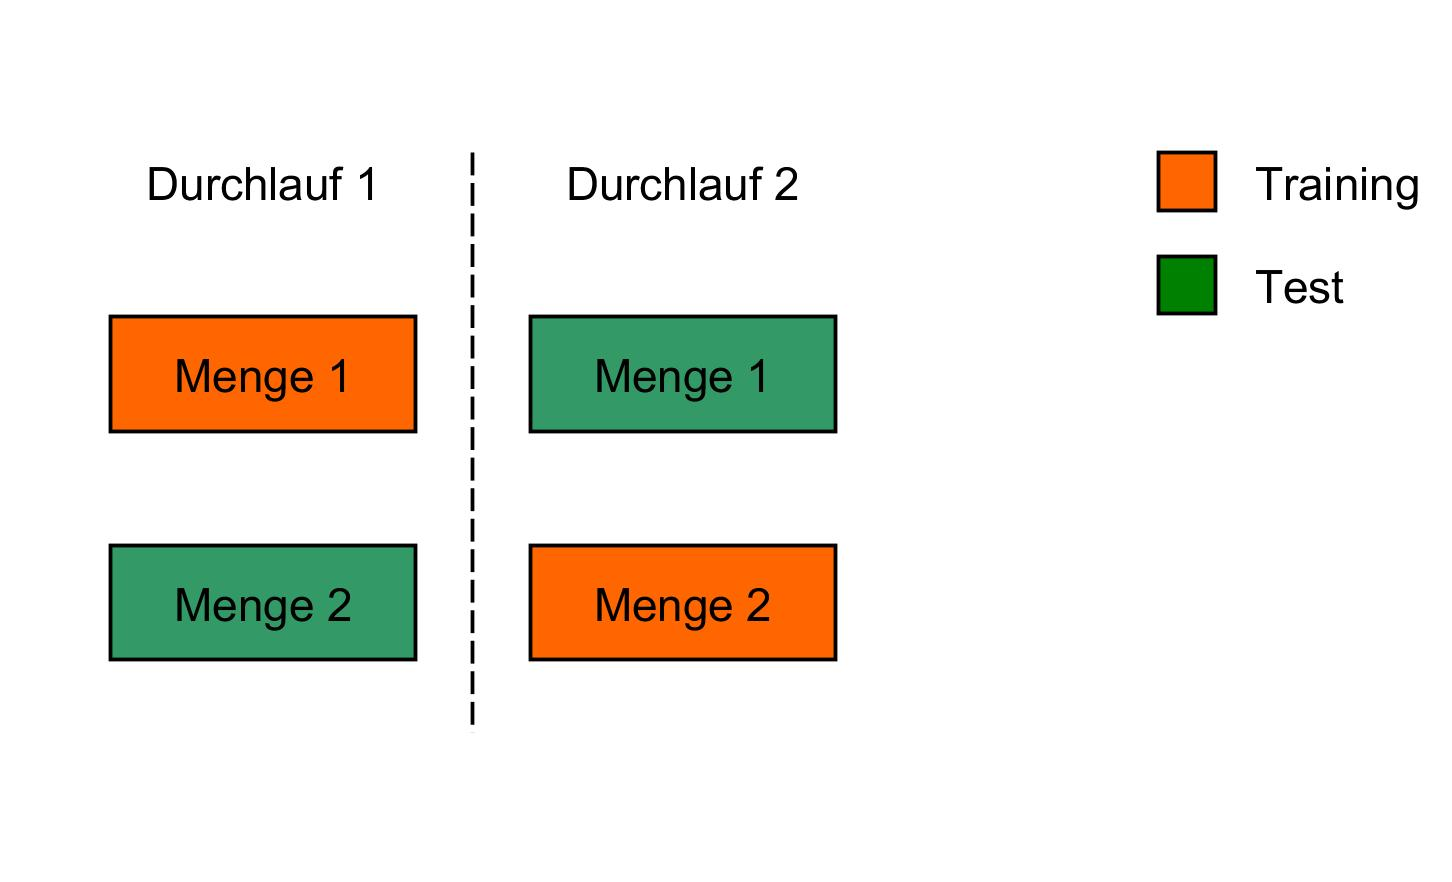
\includegraphics[scale=0.18]{bilder/cv.jpg}
		\caption{Zweifache Kreuzvalidierung}\label{CV}
	\end{center}
\end{figure}\\
Bei diesem Verfahren wird der Datensatz in zwei gleich große Mengen aufgeteilt (siehe Abbildung \ref{CV}). Die Stratifizierung bedeutet in diesem Zusammenhang, dass die Verteilung der Troll-Tweets und Nichttroll-Tweets in den beiden neu entstehenden Mengen genau wiederhergestellt wird. Im Folgenden wird dann in zwei Durchläufen eines Algorithmus wechselseitig jede der zwei Mengen einmal als Trainings- und einmal als Testmenge verwendet. Das Ergebnis für eine Hyperparameterkombination wird dann aus den Mittelwerten der beiden Durchläufe gebildet.
\subsection{Erklärte Varianz}
Ein Hyperparameter, der grundsätzlich auch in der Rastersuche mit berücksichtigt werden kann, ist das Level der Dimensionalitäsreduktion. Dies bringt jedoch einen fundamentalen Konflikt mit sich: Das Testen von mehreren Werten für die Dimensionen würde gleichsam ein Vielfaches an Ausführungen und damit eine deutlich gesteigerte Laufzeit mit sich bringen. Andererseits liefern mehr Vektorkomponenten auch mehr Informationsgehalt (eine größere Varianz) und damit bessere Ergebnisse, die auch interessant für die Optimierung sind. Letztere Proportionalität ermöglicht aber auch eine alternative Vorgehensweise: Man kann das Reduktionslevel $d$ für alle Ausführungen konstant wählen. In diesem Fall ist es entscheidend, ein $d$ zu wählen, was den Anforderungen der Laufzeit und der Qualität gerecht werden kann. Wie in Kapitel \ref{dim-red} beschrieben, kann der Informationsgehalt der einzelnen Vektorkomponenten im Zuge einer Hauptkomponentenanalyse oder einer Singulärwertzerlegung ermittelt werden. Man spricht hier von der durch eine Komponente \textbf{erklärten Varianz}.
\begin{figure}[htb]
	\begin{center}
		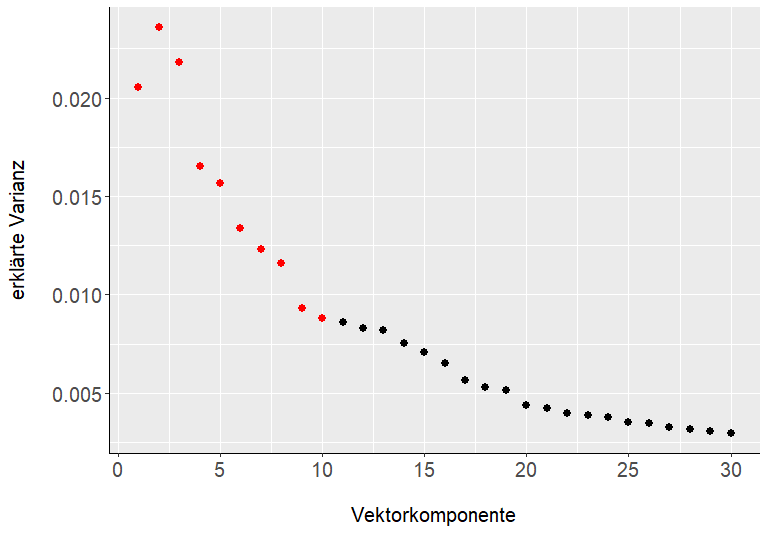
\includegraphics[width=0.85\textwidth]{bilder/expvar.png}
		\caption{Erklärte Varianz der Komponenten}\label{expvar}
	\end{center}
\end{figure}\\
Abbildung \ref{expvar} zeigt nun die 30 höchsten Werte der erklärten Varianz nach einer Singulärwertzerlegung der Vektoren des Datensatzes. Demnach erklären 3 Komponenten über 2\% der Varianz, 5 Komponenten zwischen 2 und 1\% der Varianz und der Rest die übrige Varianz. Kumuliert man diese Werte, werden durch die besten 10 Komponenten (rot) 15\% der Varianz erklärt. Dies ist für die geringe Anzahl der Komponenten ein vertretbarer Informationsgehalt. Da $d = 10$ gleichzeitig ebenfalls laufzeitverträglich ist, wird dieser Wert konstant für alle nachfolgenden Anwendungen gewählt.
\subsection{Implementierung} 
Zwecks Nachvollziehbarkeit und Transparenz soll an dieser Stelle kurz auf die parallel erfolgte praktische Anwendung der beschriebenen Techniken eingegangen werden.\\
Im Rahmen dieser Abschlussarbeit wurde ein Kommandozeilen-Tool namens \glqq TrollDetector\grqq{} \footnote{\url{https://github.com/rokoe102/trolldetector}} in der Programmiersprache Python entwickelt. Dieses hat mehrere Funktionen. Zum einen ist damit möglich, ein beliebiges Klassifikationsverfahren mit selbst gewählten Hyperparametern auf den Datensatz anzuwenden. Dies geschieht nach dem bereits erwähnten \glqq Train-and-Test\grqq-Verfahren. Hier sind auch Merkmalsextraktion (z.B. TF vs. TF-IDF) und Dimensionalitätsreduktion direkt steuerbar.\\
Eine weitere Funktion ist die Hyperparameteroptimierung für jedes Verfahren mit anschließender Auswertung der Ergebnisse. Für die Optimierung wird eine Rastersuche mit Kreuzvalidierung verwendet.\\
Schließlich ist es mit dem Programm noch möglich, einen Vergleich der fünf Klassifikatoren anzustellen. Die voreingestellten Hyperparameter sind jene, welche bei der Hyperparameteroptimierung am besten abgeschnitten haben, sodass eine Vergleichbarkeit hergestellt wird.\\
Zur Verarbeitung und Klassifikation des Datensatzes wurden ausschließlich Klassen und Funktionen aus der \glqq scikit-learn\grqq-Bibliothek von \citet{scikit-learn} verwendet.\\
\pagebreak